\documentclass[a4paper,12pt]{article}
\usepackage[bahasa]{babel}
\usepackage{graphicx}
\usepackage{multirow}
\usepackage{enumitem}
\usepackage{listings}
\usepackage{adjustbox}
\graphicspath{ {./img/} }
\begin{document}
\title{Laporan Praktikum Statistika Pertemuan 9}
%\author{Aldzikri Dwijayanto Prathama \\ {\small 195410189}}
\author{Aldzikri Dwijayanto Prathama 
	\\195410189}
\makeatletter
\begin{titlepage}
	\begin{center}
		{\huge \bfseries \@title }\\[14ex]
		
\includegraphics[scale=.8]{logo}\\[4ex]
		{\large \@author}\\[20ex]
		{\large \bfseries {SEKOLAH TINGGI MANAJEMEN INFORMATIKA DAN KOMPUTER
				AKAKOM YOGYAKARTA}}
	\end{center}


%{\large \@date} 
\end{titlepage}
\makeatother
%\maketitle
\newpage
\tableofcontents
\newpage
\section{Pembahasan}
\subsection{Praktik}
\subsubsection{Praktik 1}
\paragraph{}
Pada praktik pertama dilakukan penghitungan terhadap keuntungan bersih pertahun dari 50 perusahaan batik di Yogyakarta, datanya adalah sebagai berikut: 60 33 85 52 65 77 84 65 57 77 71 81 35 50 38 64 74 41 68 54 41 41 61 91 55 73 54 53 45 77
\begin{center}
	
\includegraphics[scale=.5]{1}
\end{center}
\begin{enumerate}[label=\alph*.]
	\item Kuartil merupakan ukuran letak yang membagi data yang sudah diurutkan menjadi empat bagian sama banyak, masing-masing bagian mempunyai 25\% data.
	Kelompok data memiliki 3 kuartil yakni kuartil bawah (Q$_{1}$), kuartil tengah atau median (Q$_{2}$), Quartil atas (Q$_{3}$). 
	\\Untuk menentukan Q$_{1}$, Q$_{2}$, dan Q$_{3}$ dari data keuntungan bersih perusahaan batik di Yogyakarta, pertama-tama masukkan data ke dalam variabel terlebih dahulu\\
	\texttt{x = c(60,33,85,52,65,77,84,65,57,77,71,81,35,50,38,64,74\\,41,68,54,41,41,61,91,55,73,54,53,45,77)\\}
	Setelah data dimasukkan ke variabel x, tentukan kuartil dengan fungsi quantile\\
	\texttt{quantile(x, probs=seq(0,1,0.25))\\}
	kuartil terletak di 25\%, 50\%, dan 75\% dari data, itu berarti nilai Q$_{1}$ nya adalah 50,50 , Q$_{2}$nya adalah 60,50, sedangkan Q$_{3}$nya adalah 73,75
	
	\item Desil merupakan  ukuran letak yang membagi data yang sudah diurutkan dari terkecil hingga terbesar menjadi sepuluh bagian sama banyak. Jadi masing-masing bagian memiliki 10 \% data keseluruhan dan memiliki 9 nilai desil.\\
	untuk menentukan D$_{4}$ dari data keuntungan bersih perusahaan batik di Yogyakarta, masukkan data ke dalam variabel terlebih dahulu\\
	\texttt{x = c(60,33,85,52,65,77,84,65,57,77,71,81,35,50,38,64,74\\,41,68,54,41,41,61,91,55,73,54,53,45,77)\\}
	Setelah data dimasukkan ke variabel x, tentukan desil dengan fungsi quantile, karena masing-masing bagian desil memiliki 10\% data keselurahan maka D$_{4}$ = 10\% * 4, maka nilai di probs adalah 0.4 maka digunakan perintah\\
	\texttt{quantile(x, probs=seq(0,4))\\}
	dari outpuynya terlihat bahwa D$_{4}$ memiliki nilai 54,6
	
	\item Persentil adalah ukuran letak yang membagi kumpulan data yang sudah diurutkan menjadi 100 bagian sama banyak dan tiap persentil  memiliki bagian 1\% data serta sekumpulan data terdapat 99 buah persentil.\\
	Untuk menentukan P$_{45}$ dari data keuntungan bersih perusahaan batik di Yogyakarta, masukkan data ke dalam variabel terlebih dahulu\\
	\texttt{x = c(60,33,85,52,65,77,84,65,57,77,71,81,35,50,38,64,74\\,41,68,54,41,41,61,91,55,73,54,53,45,77)\\}
	Setelah data dimasukkan ke variabel x, tentukan persentil dengan fungsi quantile, karena yang dicari adalah P$_{45}$, maka nilai di probs adalah 0.45 maka digunakan perintah\\
	\texttt{quantile(x, probs=seq(0,45))\\}
	dari outpuynya terlihat bahwa P$_{45}$ memiliki nilai 57,15
	
	\item Ukuran kemiringan adalah ukuran yang menyatakan sebuah model distribusi yang mempunyai kemiringan tertentu. Apabila diketahui besarnya nilai ukuran ini maka dapat diketahui pula bagaimana model distribusinya, apakah distribusi itu simetrik, positif, atau negatif.\\
	Untuk menentukan kemiringan dari data keuntungan bersih perusahaan batik di Yogyakarta, masukkan data ke dalam variabel terlebih dahulu\\
	\texttt{x = c(60,33,85,52,65,77,84,65,57,77,71,81,35,50,38,64,74\\,41,68,54,41,41,61,91,55,73,54,53,45,77)\\}
	Setelah data dimasukkan ke variabel x,tentukan koefisien kemiringan dengan fungsi describe yang terdapat dalam package psych, dengan perintah:\\
	\texttt{describe(x)}\\
	Nilai koefisien kemiringan terdapat pada kolom skew, jadi dari output di atas terlihat koefisien kemiringan dari data keuntungan perusahaan batik adalah 0,01 , dan kemiringan dari distribusi data positif. Artinya keuntungan pedagang  di rekord awal lebih tinggi dari pada record akhir.
	
	\item Ukuran keruncingan adalah kepuncakan dari suatu distribusi, biasanya diambil relatif terhadap distribusi normal. Sebuah distribusi yang mempunyai puncak relatif relatif tinggi dinamakan dinamakan leptokurtik leptokurtik, sebuah distribusi mempunyai puncak mendatar dinamakan platikurtik, distribusi normal yang puncaknya tidak terlalu tinggi atau tidak mendatar dinamakan mesokurtik.\\
	Untuk menentukan nilai koefisien kurtosis dari data keuntungan bersih perusahaan batik di Yogyakarta, masukkan data ke dalam variabel terlebih dahulu\\
	\texttt{x = c(60,33,85,52,65,77,84,65,57,77,71,81,35,50,38,64,74\\,41,68,54,41,41,61,91,55,73,54,53,45,77)\\}
	Setelah data dimasukkan ke variabel x,tentukan koefisien kurtosis dengan fungsi describe yang terdapat dalam package psych, dengan perintah:\\
	\texttt{describe(x)}\\
	Nilai koefisien kurtosis terdapat pada kolom kurtosis, jadi dari output di atas terlihat koefisien kurtosis dari data keuntungan perusahaan batik adalah -1.14 , dan karena nilai koefisien kurtosisnya < 0,263 maka distribusinya adalah platikurtik, artinya keuntungan dari pedagang batik tersebut cenderung hampir sama.
	
\end{enumerate}

\newpage

\subsubsection{Praktik 2}
Misalkan Xi adalah banyaknya penjualan beras (ton/bulan) dari dua pedagang beras (X1 dan X2), dari  Bulan Januari sampai  Desember\\ 
Pedagang (X1) : 10, 8, 6, 3, 6, 5, 6, 12, 4, 20, 2, 15\\
Pedagang (X2) : 8, 6, 9, 10, 12, 12, 13, 9, 7, 5, 14, 4

\begin{center}
	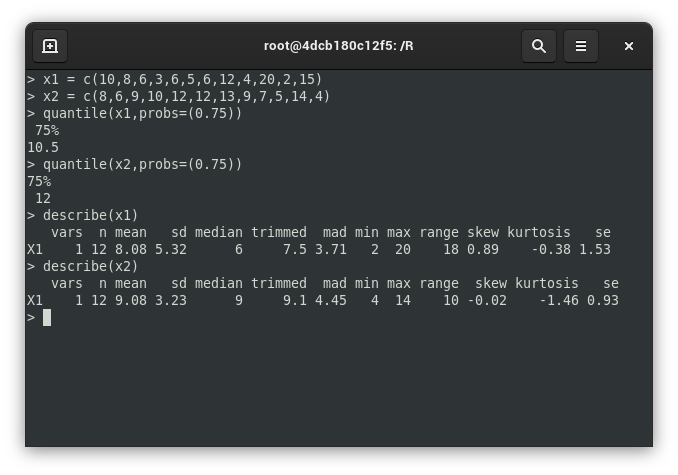
\includegraphics[scale=.5]{2}
\end{center}

\begin{enumerate}[label=\alph*.]
	\item Untuk menentukan nilai penjualan sampai kuartal ke-3 (Q3) dari kedua pedagang tersebut, masukkan data terlebih dahulu\\
	\texttt{x1 = c(10,8,6,3,6,5,6,12,4,20,2,15)}\\
	\texttt{x2 = c(8,6,9,10,12,12,13,9,7,5,14,4)}\\
	Lalu tentukan kuartal ke-3 (Q$_{3}$) masing-masing data dengan fungsi kuantile\\
	untuk x1\\
	\texttt{quantile(x1,probs=(0.75))}
	untuk x2\\
	\texttt{quantile(x2,probs=(0.75))}\\
	dari outputnya nilai penjualan sampai kuartal ke-3 (Q3) dari pedagang X1 = 10.5 , X2 = 12. Terlihat pedagang X2 nilia penjualan sampai kuartal ke-3 lebih tinggi.
	
	\item Untuk menentukan nilai kemiringan penjualan dari kedua pedagang tersebut, masukkan data terlebih dahulu\\
	\texttt{x1 = c(10,8,6,3,6,5,6,12,4,20,2,15)}\\
	\texttt{x2 = c(8,6,9,10,12,12,13,9,7,5,14,4)}\\
	Lalu tentukan kemiringan dengan fungsi describe yang ada pada library psych\\
	Untuk x1\\
	\texttt{describe(x1)\\}
	Untuk x2\\
	\texttt{describe(x2)\\}
	Dari ouputnya terlihat kemiringan dari distribusi data pedagang X1 = 0.89 dan X2 = -0.02. Kemiringan distribusi penjualan pedagang X1 positif artinya penjualan di bulan awal lebih tinggi dari pada bulan akhir.\\
	Sedangkan kemiringan distibusi penjualan pedagang X2 negatif artinya penjualan di bulan awal cenderung lebih rendah dari pada penjualan dibulan akhir.
	
\end{enumerate}

\subsection{Latihan}
\subsubsection{Latihan 1}
Data mengenai lama (durasi) beberapa judul film dengan data mentah sebagai berikut. 83 88 120 64 69 71 76 74 75 75 76 75 79 80 73 72 82 74 84 90 89 81 90 89 81 81 90 79 92 82 89 82 74 86
\begin{center}
	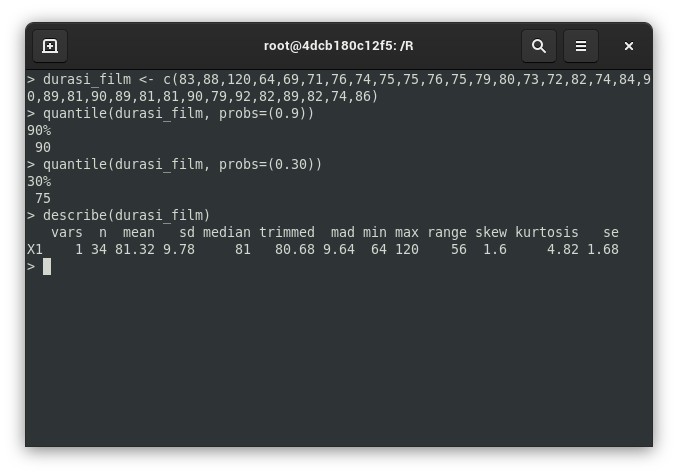
\includegraphics[scale=.5]{lat1}
\end{center}
\begin{enumerate}[label=\alph*.]
	\item untuk menentukan D$_{9}$ dari data di atas, masukkan data ke dalam variabel terlebih dahulu\\
	\texttt{x = durasi\_film <- c(83,88,120,64,69,71,76,74,75,75,76,75,79\\
		,80,73,72,82,74,84,90,89,81,90,89,81,81,90,79,92,82,89,82,74,86)\\}
	Setelah data dimasukkan ke variabel durasi\_film, tentukan desil dengan fungsi quantile, karena masing-masing bagian desil memiliki 10\% dari data keselurahan maka D$_{9}$ = 10\% * 9, maka nilai di probs adalah 0.9 maka digunakan perintah\\
	\texttt{quantile(durasi\_film, probs=seq(0,9))\\}
	dari outpuynya terlihat bahwa D$_{9}$ memiliki nilai 90
	
	\item Untuk menentukan P$_{45}$ dari data durasi film, masukkan data ke dalam variabel terlebih dahulu\\
	\texttt{x = durasi\_film <- c(83,88,120,64,69,71,76,74,75,75,76,75,79\\
		,80,73,72,82,74,84,90,89,81,90,89,81,81,90,79,92,82,89,82,74,86)\\}
	Setelah data dimasukkan ke variabel durasi\_film, tentukan persentil dengan fungsi quantile, karena yang dicari adalah P$_{30}$, maka nilai di probs adalah 0.30 maka digunakan perintah\\
	\texttt{quantile(durasi\_film, probs=seq(0,30))\\}
	dari outpuynya terlihat bahwa P$_{45}$ memiliki nilai 75
	
	\item Untuk menentukan kemiringan dari data durasi\_film, masukkan data ke dalam variabel terlebih dahulu\\
	\texttt{x = durasi\_film <- c(83,88,120,64,69,71,76,74,75,75,76,75,79,\\
		80,73,72,82,74,84,90,89,81,90,89,81,81,90,79,92,82,89,82,74,86)\\}
	Setelah data dimasukkan ke variabel durasi\_film, tentukan koefisien kemiringan dengan fungsi describe yang terdapat dalam package psych, dengan perintah:\\
	\texttt{describe(durasi\_film)}\\
	Nilai koefisien kemiringan terdapat pada kolom skew, jadi dari output di atas terlihat koefisien kemiringan dari data durasi\_film adalah 1,0 , dan kemiringan dari distribusi data positif. Artinya durasi\_film  di rekord awal lebih tinggi dari pada record akhir.
	
	\item Untuk menentukan nilai koefisien kurtosis dari data durasi\_film, masukkan data ke dalam variabel terlebih dahulu\\
	\texttt{x = durasi\_film <- c(83,88,120,64,69,71,76,74,75,75,76,75,79,\\
		80,73,72,82,74,84,90,89,81,90,89,81,81,90,79,92,82,89,82,74,86)\\}
	Setelah data dimasukkan ke variabel durasi\_film,tentukan koefisien kurtosis dengan fungsi describe yang terdapat dalam package psych, dengan perintah:\\
	\texttt{describe(durasi\_film)}\\
	Nilai koefisien kurtosis terdapat pada kolom kurtosis, jadi dari output di atas terlihat koefisien kurtosis dari data durasi\_film adalah 4.82 , dan karena nilai koefisien kurtosisnya kurtosisnya > 0,263 maka distribusinya adalah leptokurtik. 
\end{enumerate}

\subsubsection{Latihan 2}
Dari catatan sebuah rumah sakit bersalin diperoleh data tentang dan berat badan bayi yang dilahirkan di rumah sakit A dan B tersebut. Dari sampel random sebanyak 20 orang bayi, berat badannya sebagai berikut (kg)\\ 
rumah sakit A  : 2.5, 3, 4, 2.4, 3.6, 3, 2.8, 2.3,  2.9\\
rumah sakit B : 3.5, 4.1, 3.4, 2.8, 3, 3.5, 3.2, 2.6, 3.3, 2.8, 3.7, 3.7, 2.9, 2.6
\begin{center}
	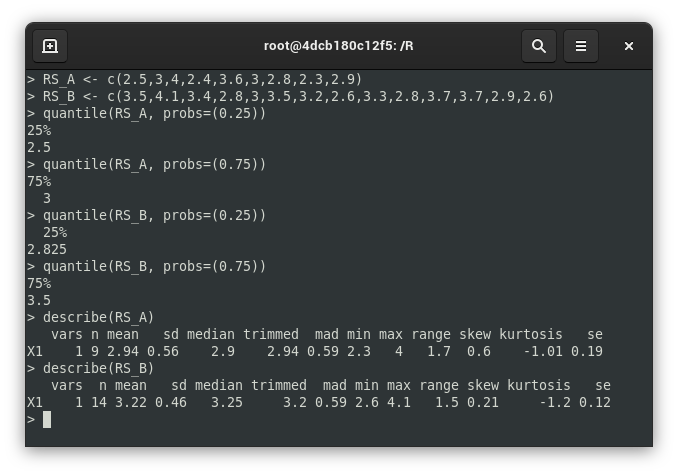
\includegraphics[scale=.5]{lat2}
\end{center}
\begin{enumerate}[label=\alph*.]
	\item Untuk menentukan Q$_{1}$ dan Q$_{3}$ dari data kedua rumah sakit tersebut di atas, masukkan data ke dalam variabel terlebih dahulu\\
	\texttt{RS\_A <- c(2.5,3,4,2.4,3.6,3,2.8,2.3,2.9)}\\
	\texttt{RS\_B <- c(3.5,4.1,3.4,2.8,3,3.5,3.2,2.6,3.3,2.8,3.7,3.7,2.9,2.6)}\\
	Lalu tentukan Q$_{1}$ dan Q$_{3}$ dengan fungsi quantile\\
	Untuk menentukan Q$_{1}$ dan Q$_{3}$ RS A\\
	\texttt{quantile(RS\_A, probs=(0.25))}\\
	\texttt{quantile(RS\_A, probs=(0.75))}\\
	Sedangkan untuk menentukan Q$_{1}$ dan Q$_{3}$ RS B\\
	\texttt{quantile(RS\_B, probs=(0.25))}\\
	\texttt{quantile(RS\_B, probs=(0.75))}\\
	Dari output di atas RS A memiliki nilai Q$_{1}$ = 2,5 dan Q$_{3}$ = 3. Sedangkan RS B memiliki nilai Q$_{1}$ = 2,825 dan Q$_{3}$ = 3,5.
	
	\item Untuk menentukan keruncingan dan kemiringan dari data kedua rumah sakit tersebut, gunakan fungsi describe dari library psych.\\
	Untuk rumah sakit A\\
	\texttt{describe(RS\_A)}\\
	Sedangkan untuk rumah sakit B\\ 
	\texttt{describe(RS\_B)}\\
	Dari outputnya terihat Rumah sakit A memiliki keruncingan -1,01, karena nilai koefisien kurtosisnya < 0,263 maka distribusinya adalah platikurtik. Sedangkan kermiringannya 0,6.\\
	Sedangkan untuk Rumah sakit B memiliki keruncingan -1,2 , karena nilai koefisien kurtosisnya < 0,263 maka distribusinya adalah platikurtik. Sedangkan kermiringannya 0,21.
\end{enumerate}

\subsection{Latihan}
\subsubsection{Latihan 1}
Perhatikan data berikut
\begin{table}[!ht]
	\begin{tabular}{|l|l|l|}
		\hline
		Panjang bayi            & Umur       & Bobot lahir \\ \hline
		(\textbackslash{}cm), y & (hari), x1 & (kg), x2    \\ \hline
		57.5                    & 78         & 2.75        \\ \hline
		52.8                    & 69         & 2.15        \\ \hline
		61.3                    & 77         & 4.41        \\ \hline
		67                      & 88         & 5.52        \\ \hline
		53.5                    & 67         & 3.21        \\ \hline
		62.7                    & 80         & 4.32        \\ \hline
		56.2                    & 74         & 2.31        \\ \hline
		68.5                    & 94         & 4.3         \\ \hline
		69.2                    & 102        & 3.71        \\ \hline
	\end{tabular}
\end{table}

\begin{enumerate}[label=\alph*.]
	\item \begin{minipage}[t]{\linewidth}
		\raggedright
		\adjustbox{valign=t}{%
			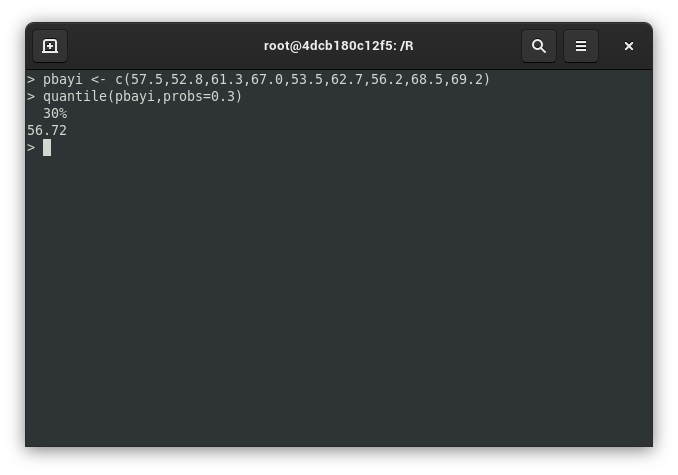
\includegraphics[width=.75\linewidth]{tugas1a}%
		}
	\end{minipage}
	Untuk menentukan D$_{3}$ dari data panjang bayi, pertama masukkan data\\
	\texttt{pbayi <- c(57.5,52.8,61.3,67.0,53.5,62.7,56.2,68.5,69.2)\\}
	Lalu tentukan D$_{3}$ dengan perintah\\
	\texttt{quantile(pbayi,probs=(0.3))\\}
	Dari outputnya terlihat nilai D$_{3}$ data dari panjang bayi memiliki nilai 56,72
	
	\item 
	\begin{minipage}[t]{\linewidth}
		\raggedright
		\adjustbox{valign=t}{
			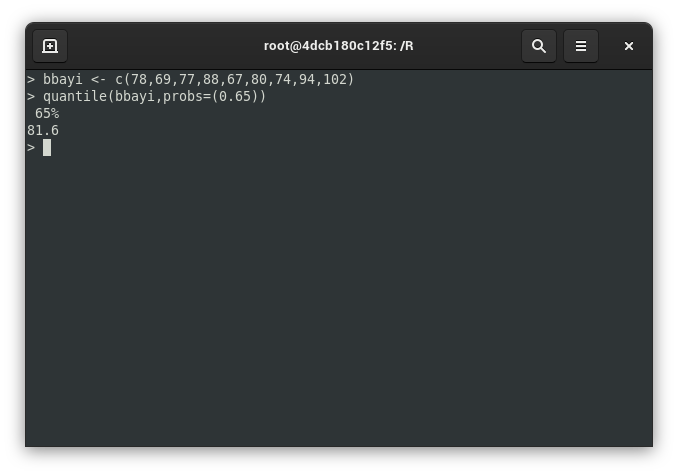
\includegraphics[width=.75\linewidth]{tugas1b}%
		}
	\end{minipage}
	Untuk menentukan P$_{65}$ dari data panjang bayi, pertama masukkan data\\
	\texttt{bbayi <- c(78,69,77,88,67,80,74,94,102)\\}
	Lalu tentukan P$_{65}$ dengan perintah\\
	\texttt{quantile(bbayi,probs=(0.65))\\}
	Dari outputnya terlihat nilai P$_{65}$ data dari panjang bayi memiliki nilai 81,6
	
	\item 
	\begin{minipage}[t]{\linewidth}
		\raggedright
		\adjustbox{valign=t}{
			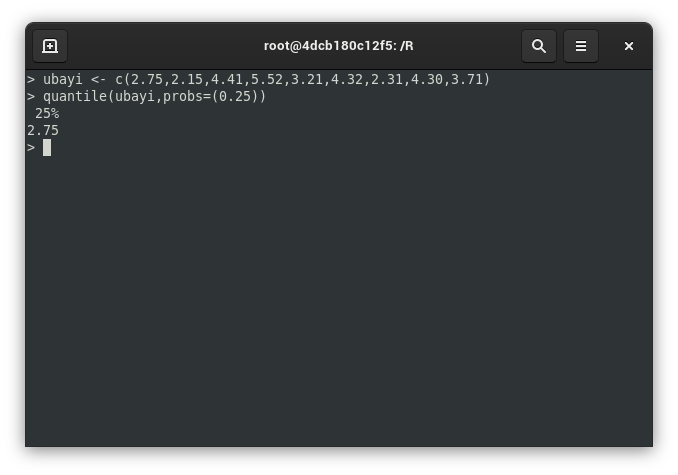
\includegraphics[width=.75\linewidth]{tugas1c}%
		}
	\end{minipage}
	Untuk menentukan Q$_{1}$ dari data panjang bayi, pertama masukkan data\\
	\texttt{ubayi <- c(2.75,2.15,4.41,5.52,3.21,4.32,2.31,4.30,3.71)\\}
	Lalu tentukan Q$_{1}$ dengan perintah\\
	\texttt{quantile(ubayi,probs=(0.25))\\}
	Dari outputnya terlihat nilai Q$_{1}$ data dari panjang bayi memiliki nilai 2,75.
	
	\item 
	\begin{minipage}[t]{\linewidth}
		\raggedright
		\adjustbox{valign=t}{
			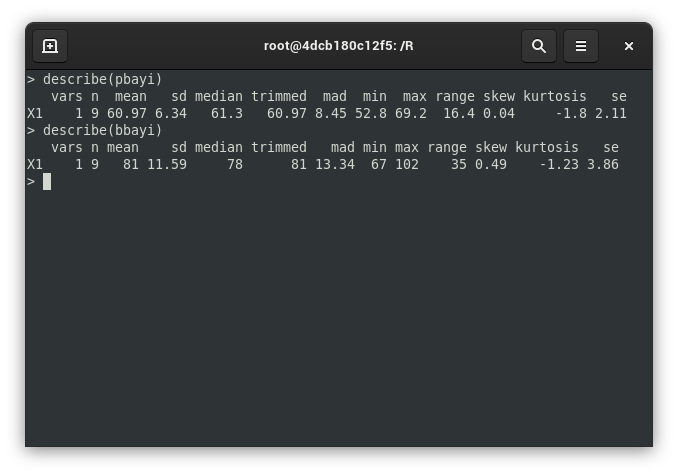
\includegraphics[width=.75\linewidth]{tugas1d}%
		}
	\end{minipage}
	Dari output di atas, data dari panjang bayi memiliki nilai kemiringan 0,04 , sedangkan data dari bobot bayi memiliki nilai kemiringan 0,49.  
			
\end{enumerate}

\newpage

\subsubsection{Latihan 2}
Diberikan data nilai mahasiswa sebagai berikut: 68 84 75 82 68 90 62 88 76 93 73 79 88 73 60 93 71 59 85 75 61 65 75 87 74 62 95 78 63 72

\begin{enumerate}[label=\alph*.]
	\item 
	\begin{minipage}[t]{\linewidth}
		\raggedright
		\adjustbox{valign=t}{
			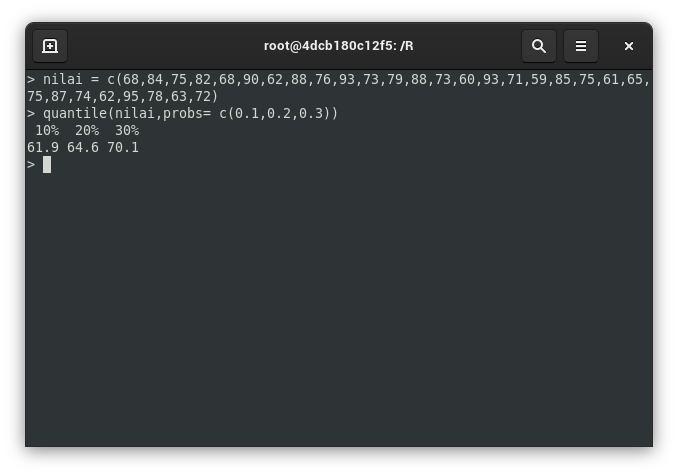
\includegraphics[width=.75\linewidth]{tugas2a}%
		}
	\end{minipage}
	untuk menentukan D$_{1}$, D$_{2}$, dan D$_{3}$, pertama masukkan data\\
	\texttt{nilai = c(68,84,75,82,68,90,62,88,76,93,73,79,88,73,60,93\\
		,71,59,85,75,61,65,75,87,74,62,95,78,63,72)}\\
	Lalu tentukan D$_{1}$, D$_{2}$, dan D$_{3}$ dengan perintah\\
	\texttt{quantile(nilai,probs= c(0.1,0.2,0.3))\\}
	dari output di atas terlihat D$_{1}$ memiliki nilai 61,9, D$_{2}$ memiliki nilai 64,6, sedangkan D$_{3}$ memiliki nilai 70,1.
\end{enumerate}
\end{document}